 \documentclass[conference]{IEEEtran}
\usepackage{subfig}
\usepackage{wrapfig}
 \usepackage{amsmath}
 \usepackage{url}
 \usepackage{pifont}
\usepackage{rotating}
%\usepackage{balance} 
\usepackage{color, colortbl}
\usepackage{graphicx}
\usepackage{algorithmicx}
\usepackage{program}
\usepackage{cite}
\usepackage{alltt}
\newcommand{\eq}[1]{Equation~\ref{eq:#1}}
\newcommand{\bi}{\begin{itemize}}
\newcommand{\ei}{\end{itemize}}
\newcommand{\be}{\begin{enumerate}}
\newcommand{\ee}{\end{enumerate}}
\newcommand{\tion}[1]{\textsection\ref{sec:#1}}
\newcommand{\fig}[1]{Figure~\ref{fig:#1}}
\definecolor{lightgray}{gray}{0.975}
\usepackage{fancyvrb}
\usepackage{stfloats}
\usepackage{multirow}
\usepackage{listings}
\usepackage{amsmath} 
\DeclareMathOperator*{\argmin}{arg\,min} 
\DeclareMathOperator*{\argmax}{arg\,max} 


\definecolor{darkgreen}{rgb}{0,0.3,0}

\usepackage[table]{xcolor}
\definecolor{Gray}{rgb}{0.88,1,1}
\definecolor{Gray}{gray}{0.85}
\definecolor{Blue}{RGB}{0,29,193}
\newcommand{\G}{\cellcolor{green}}
\newcommand{\Y}{\cellcolor{yellow}}


\definecolor{MyDarkBlue}{rgb}{0,0.08,0.45} 
\newenvironment{changed}{\par\color{MyDarkBlue}}{\par}

\newcommand{\ADD}[1]{\textcolor{MyDarkBlue}{{\bf #1}}}
\newcommand{\addit}[1]{\begin{changed}\input{#1}\end{changed}}

\usepackage{color}
\usepackage{listings}
\usepackage{setspace}

\definecolor{Gray}{gray}{0.9}
\newcommand{\kw}[1]{\textit{#1}}
\newcommand{\quart}[4]{\begin{picture}(75,6)
  {\color{black}\put(#3,3){\circle*{4}}\put(#1,3){\line(1,0){#2}}}\end{picture}}
% New Commands

\definecolor{Code}{rgb}{0,0,0}
\definecolor{Decorators}{rgb}{0.5,0.5,0.5}
\definecolor{Numbers}{rgb}{0.5,0,0}
\definecolor{MatchingBrackets}{rgb}{0.25,0.5,0.5}
\definecolor{Keywords}{rgb}{0,0,1}
\definecolor{self}{rgb}{0,0,0}
\definecolor{Strings}{rgb}{0,0.63,0}
\definecolor{Comments}{rgb}{0,0.63,1}
\definecolor{Backquotes}{rgb}{0,0,0}
\definecolor{Classname}{rgb}{0,0,0}
\definecolor{FunctionName}{rgb}{0,0,0}
\definecolor{Operators}{rgb}{0,0,0}
\definecolor{Background}{rgb}{1,1,1}

\lstnewenvironment{python}[1][]{
\lstset{
mathescape,
numbers=#1,
numberstyle=\footnotesize,
numbersep=0.5em,
xleftmargin=0em,
framextopmargin=2em,
framexbottommargin=2em,
showspaces=false,
showtabs=false,
showstringspaces=false,
tabsize=2,
% Basic
basicstyle=\ttfamily\small\setstretch{0.8},
backgroundcolor=\color{Background},
language=Python,
% Comments
commentstyle=\color{Comments}\slshape,
% Strings
stringstyle=\color{Strings},
morecomment=[s][\color{Strings}]{"""}{"""},
morecomment=[s][\color{Strings}]{'''}{'''},
% keywords
morekeywords={[1]import,from,class,def,for,while,if,is,in,elif,else,not,and,or,print,break,continue,return,True,False,None,access,as,,del,except,exec,finally,global,import,lambda,pass,print,raise,try,assert, dot, norm, zip, sorted},
keywordstyle={[1]\color{Code}\bfseries},
% additional keywords
morekeywords={[3]fastmap, project, furthest, split, where,clusterer, getExemplar, projection, mutate, WHAT, knn},
keywordstyle={[3]\color{Keywords}\bfseries},
morekeywords={[2]@invariant},
keywordstyle={[2]\color{Decorators}\slshape},
emph={self},
emphstyle={\color{self}\slshape},
%
}}{}


\begin{document}
  \title{``Don't tell me what it is, tell me what to do'':\\Instance-Based Planning for Actionable Analytics}
  
  % make the title area
  \maketitle
  
  
  \begin{abstract}
 
  \end{abstract}
  \begin{IEEEkeywords}
    defect prediction, CART
  \end{IEEEkeywords}
  
\section{Introduction}
{\bf RQ1: Can Instance-based Learning techniques be used to create Planning tools that can better analyse software defect?} 


{\bf RQ2: Can lessons learnt from local search operators be useful for generating solutions that can be used to mitigate defects in software systems?} 

{\bf RQ3: Can such instance-based planners be applied to other software engineering paradigms?}
We check if the proposed instance-based planner is applicable to performance prediction.

\section{Motivating Example}
\section{Background}
\section{Instance Based Learning}

Assessing the quality of solutions to a real-world problem can be extremely hard~\cite{menzies2005xomo}. In several software engineering applications, researchers have models that can emulate the problem, for instance there is the COCOMO effort model~\cite[p29-57]{boehm2009software}, the COQUALMO defect model~\cite[p254-268]{boehm2009software}, Madachy’s schedule risk model~\cite[p284-291]{boehm2009software}, to name a few. Using these models it is possible to examine several scenarios in a short period of time, and this can be done in a reproducible manner. However, models aren't always the solution, as we shall see. 

There exist several problems where models are hard to obtain, or the input and output are related by complex connections that simply cannot be modeled in a reliable manner, or generation of reliable models take prohibitively long ~\cite{Ludewig2003}. Software defect prediction is an excellent example of such a case. Models that incorporate all the intricate issues that may lead defects in a product is extremely hard to come by. Moreover, it has been shown that models for different regions within the same data can have very different properties \cite{localvsglobal}. This makes it extremely hard for one to design planning systems that are capable of mitigating these defects.

In this paper we propose the use of an instance based approach, an example of case based reasoning strategy, in place of the conventional model based approach. Instance based approaches have been used extensively by the effort estimation community, see~\cite{keung2008analogy, 6600685, walkerden1999empirical, shepperd1997estimating, kocaguneli2010use, some more form p1703 line 2}. This approach has been proposed as an alternative to closed form mathematical models of other modeling methods such as regression \cite{keung2008analogy}. There are several other reasons for instance based approaches being a useful tool, see~\cite{6600685}. As pointed out by~\cite{walkerden1999empirical} it can be used with partial knowledge of the target project at an early stage which could be a very useful tool in preventing software defects. Instance based approaches are also rather robust in handling cases with sparse samples \cite{1438374}. All these features are desirable and suggest that instance-based approach is a useful adjunct to traditional model based approach. 

We would like to stress that the purpose of our work is not to promote instance-based planning over model based analytics, rather it is to suggest an alternative when model based approaches cannot be used.

\subsection{Spectral Learning using WHERE}
The algorithm uses WHERE to recursively cluster the input data to identify subsets in the training data that a test instance can learn from. WHERE is a spectral learner which uses the FastMap heuristic to estimate the first principal component. It then recursively partitions the data into two halves along the Medianian point of the projection on the first principal component, terminating when a half has less than $\sqrt{N}$ items.   

\subsection{Planning changes using WHAT}
We propose the WHAT algorithm as a tool to plan changes in the original test data. Figure~\ref{fig:what} highlights the procedure by which WHAT operates. It begins by creating clusters which are generated using the WHERE algorithm discussed above. Following this, a nearest neighbour scheme is applied to identify pairs of nearby clusters. A projective plane is constructed with these clusters at the vertices to characterize the cluster pairs.

The mutation policy works by projecting the test instance onto the projective planes and identifying the the plane on which the test instance has the largest scalar projection. The planner then reflects over the vertices of the chosen hyperplane, identifying the \textit{better} vertex among the two. Now, a new instance is generated by mutating the attributes of the test instance towards the better vertex and away from the worse vertex. This process is repeated for all the test instances that are considered defective by the defect prediction scheme, discussed below.

\begin{figure}[htbp!]
\small
\begin{tabular}{|p{.95\linewidth}|}\hline
WHAT begins by \textit{clustering} the training data into similar subsets using WHERE. WHERE works as follows:
\begin{enumerate}
\item Find the two most distant points in a given population; say {\em east} and {\em west}. 
\item Draw an axis of length $c$ between the poles. 
\item Let each point be at distance $a,b$ to the {\em east,west} poles.  Using the cosine rule, project each point onto the  axis  at $x=(a^2 + c^2 - b^2)/(2c)$.  
\item Using the Medianian $x$ value, divide the population.
\item For each half that is larger than $\sqrt{N}$ of the original population, go to step 1.
\end{enumerate}

There are couple of things to note: firstly, the above algorithm requires a distance measure between sets of decisions, for this WHERE uses case-based reasoning measure defined by Aha et al.~\cite{aha91}; secondly, in step-1 a linear time heuristic called FASTMAP~\cite{fastmap} is used to find the two most distant points, this procedure is listed below:
\begin{itemize}
\item Pick a point at random; 
\item Let {\em east} be the point furthest from that point; 
\item Then {\em west} be the point furthest from {\em east}.
\end{itemize}

The final clusters that are found by WHERE are then used by WHAT as follows:
\begin{itemize}
\item For each cluster find its nearest neighbor.
\item Construct a projective plane for each cluster pair. Label the cluster pairs as {\em Good} and {\em Bad}.
\item For a test instance, project it onto the planes generated above and pick the one on which the test case has the largest projection.
\item Mutate the attributes of the test case towards the {\em Good Cluster} in that projective plane. 
\end{itemize}

Formally, WHAT can be considered as an instance based  learning scheme. And that's beacuse it builds a set of recommendations based on a given test case based on the clusters forMedian at the training stage. This is unlike a model based approach, which would have used a model to do the same~\cite{xomo}.
\\\hline
\end{tabular}
\caption{Inside WHAT}\label{fig:what}
\end{figure}

\begin{figure}
\centering
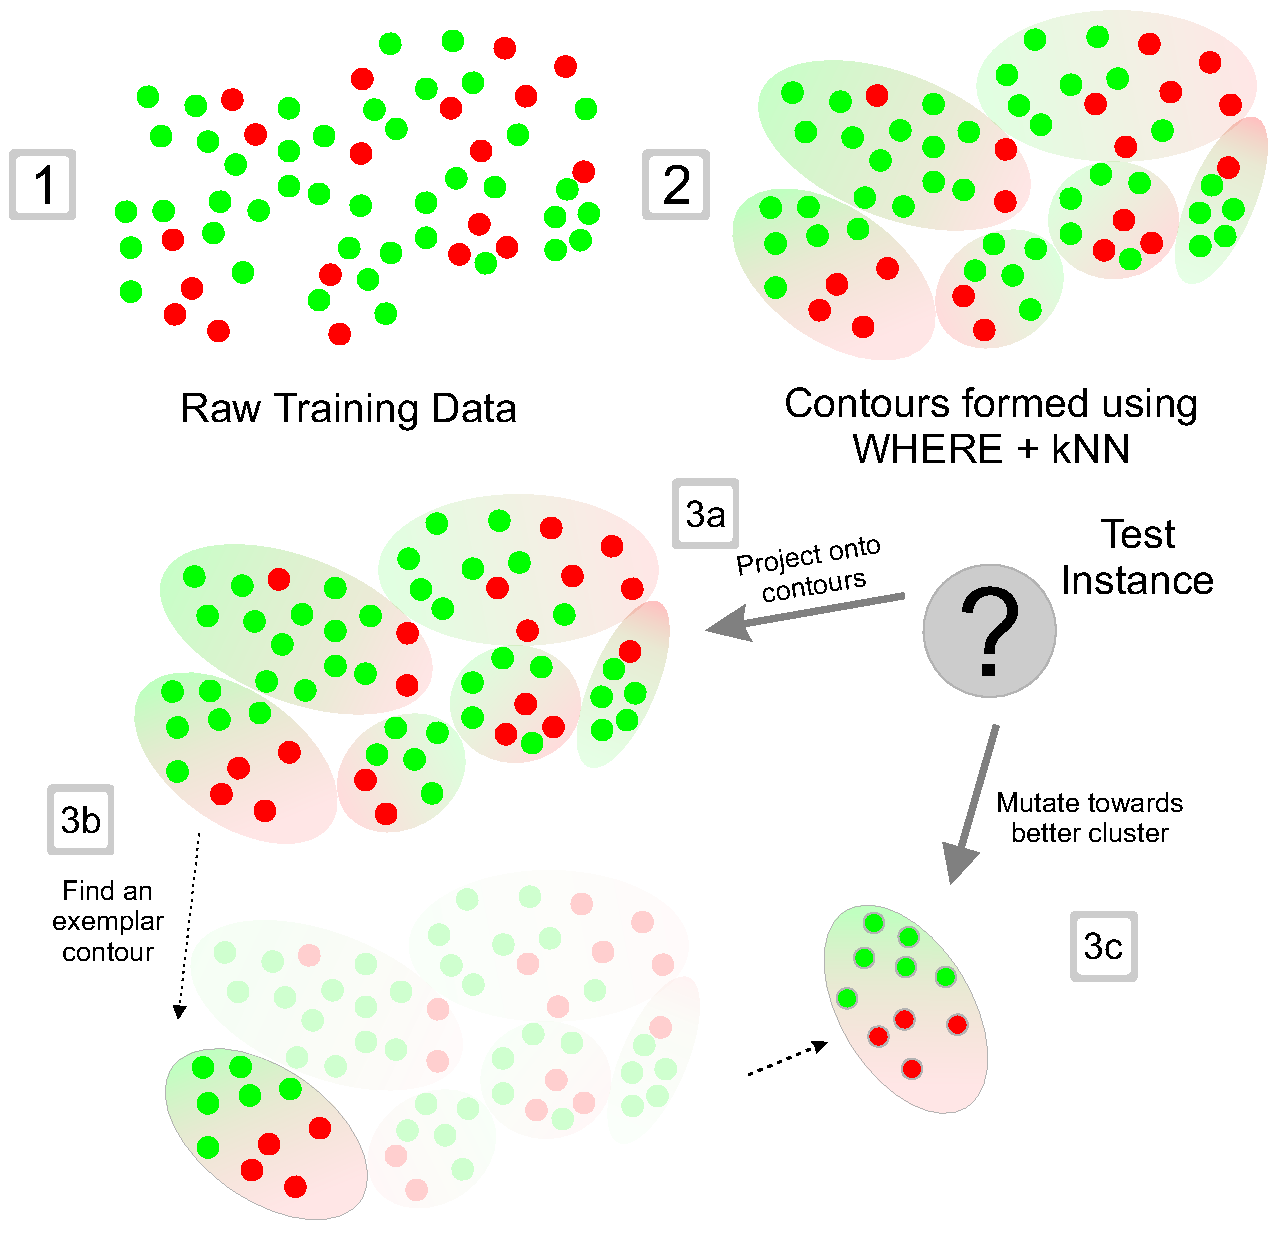
\includegraphics[width=\linewidth]{_figs/WHAT-Clusters2.pdf}
\caption{WHAT}
\label{fig:whatflow}
\end{figure}

\begin{figure}[!b]
\begin{python}[right]
def fastmap(data): 
  """Project data on a line 
     between 2 distant points
  """
  z          = random.choose(data)
  east       = furthest(z, data)
  west       = furthest(east, data)
  data.poles = (west,east)
  c          = dist(west,east)     
  for one in data.members: 
    one.pos = project(west,east,c,one)
  data = sorted(data) # sorted by 'pos'
  return split(data)

def project(west, east, c, x): 
  "Project x onto line east to west"
  a = dist(x,west)
  b = dist(x,east)
  return (a*a + c*c - b*b)/(2*c) #cosine rule

def furthest(x,data): 
  # what is furthest from x?
  out, max = x,0
  for y in data:
    d = dist(x,y)
    if d > max: out, max = y, d
  return out

def split(data): # Split at median
   mid = len(data)/2; 
  return data[mid:], data[:mid]

def where(data, scores={}, 
          lvl=10000, prune=True):  
  "Recursively split data into 2 equal sizes."
  if lvl < 1: 
     return data # stop if out of levels
  leafs      = [] # Empty Set
  left,right = fastmap(data)
  west, east = data.poles
  $\omega=\sqrt{\mu}$ # enough data for recursion
  goWest = len(left) > $\omega$  
  goEast = len(right) > $\omega$ 
  if prune: # if not pruning, ignore this step
    if goEast and better(west,east,scores): 
       goEast = False 
    if goWest and better(east,west,scores): 
       goWest = False 
  if goWest:  
     leafs += where(left,  lvl - 1, prune)  
  if goEast:  
     leafs += where(right, lvl - 1, prune) 
  return leafs

\end{python}
\caption{Clustering with WHERE}
\label{fig:fastmapCode}   
\end{figure}


\begin{figure}[!t]
\begin{python}[left]
def clusterer():
 "Create clusters using WHERE"
 
def getExemplar():
  """
  Identify the contour that exemplifies
  the test Instance the most
  """
  contours = []
  ClusterRows = clusterer()
  while ClusterRows:
    one = ClusterRows.pop()
    two = knn(one, ClusterRows)[1]
    contours.append([one, two])
  return contours

def projection(one, two, three):
  "Compute projection of three on one & two"
  if one.score() > two.score():
    bad, good = one, two
  else:
    bad, good = two, one
  plane = [b - a for a, b in zip(
            bad.rep(), good.rep())]
  Norm = norm(plane)
  unitVect = [p / Norm for p in plane]
  proj = dot(three - bad.rep(), unitVect)
  return proj

def mutate(me, others):
  "Mutate 'me' towards 'others'"
  return [my + ext * (good - my) 
    	 for my, good in zip(me, others)]

def WHAT():
  contours = getExemplar()
  for rows in defectiveRows:
    vtx = sorted(
        contours,
        key=lambda F: projection(
        F[0], F[1], rows), reverse=True)[0]
    
    [good, bad] = sorted(vtx
            , key=lambda F: F.score())
    newRows.append(mutate(rows, good))
  return newRows
\end{python}
\caption{Instance-based Planning using WHAT}
\label{fig:WHAT}   
\end{figure}

\subsection{Defect Prediction}

To validate the treatments that have been suggested by our planner, we need to have defect predictors that capable of identifying if a certain module may (or may not) have a defect. A recent IEEE TSE paper by Lessmann et al.~\cite{lessmann} compared 21 different learners for software defect prediction: 
\bi
\item
{\em Statistical classifiers:}
Linear    discriminant analysis,
Quadratic discriminant analysis,
Logistic regression,
Naive Bayes,
Bayesian networks,
Least-angle regression,
Relevance vector machine,

\item
{\em Nearest neighbor methods:}
k-nearest neighbor,
K-Star

\item
{\em Neural networks:}
Multi-Layer Perceptron,
Radial bias functions,

\item
{\em Support vector machine-based classifiers:}
Support vector machine,
Lagrangian SVM
Least squares SVM,
Linear programming,
Voted perceptron,

\item
{\em Decision-tree approaches:}
C4.5,
CART,
Alternating DTs
\item
{\em Ensemble methods:}
\textbf{Random Forest},
Logistic Model Tree.
\ei

They concluded that Random Forrest was the best method, CART being the worst.

Random Forest is an ensemble learning scheme that constructs a number of decision trees at the training time, for a test instance it outputs the mode of the classes of individual tree. It's patent from how random forest operates that the prediction will suffer if there is an imbalance in classes during the training. Unfortunately, the data sets explored here do suffer from severe skewness, as highlighted in~\ref{fig:classimb}. A study conducted by Pelayo and Dick~\cite{smote2} inspected this issue. They showed that the SMOTE technique~\cite{smote} can be used to improve recognition of defect-prone modules. 

In short, SMOTE works by under-sampling the majority class and oversampling all the minority classes in the training data. We use a similar approach with one minor addition to the original algorithm. In our implementation of SMOTE we have introduced an additional step called \textit{resampling}, wherein we ensure that after we do the over/under sampling, the new training data does not have any of the original rows. The new training data merely resembles the original data. This is done as a precautionary measure, so as not to have WHAT and Random Forest train on the same training data. 
%Its worth noting that both WHAT and Random Forest require some data to train. In order to prevent the two from using the same data to train, we run SMOTE by  \textit{resampling} the classes. Re-sampling 

\begin{figure*}[htbp!]
  \renewcommand{\baselinestretch}{0.8}\begin{center}
    {\scriptsize
      \begin{tabular}{c|l|p{4.7in}}
        amc & average method complexity & e.g. number of JAVA byte codes\\\hline
        avg\_cc & average McCabe & average McCabe's cyclomatic complexity seen
        in class\\\hline
        ca & afferent couplings & how many other classes use the specific
        class. \\\hline
        cam & cohesion amongst classes & summation of number of different
        types of method parameters in every method divided by a multiplication
        of number of different method parameter types in whole class and
        number of methods. \\\hline
        cbm &coupling between methods &  total number of new/redefined methods
        to which all the inherited methods are coupled\\\hline
        cbo & coupling between objects & increased when the methods of one
        class access services of another.\\\hline
        ce & efferent couplings & how many other classes is used by the
        specific class. \\\hline
        dam & data access & ratio of the number of private (protected)
        attributes to the total number of attributes\\\hline
        dit & depth of inheritance tree &\\\hline
        ic & inheritance coupling &  number of parent classes to which a given
        class is coupled (includes counts of methods and variables inherited)
        \\\hline
        lcom & lack of cohesion in methods &number of pairs of methods that do
        not share a reference to an instance variable.\\\hline
        locm3 & another lack of cohesion measure & if $m,a$ are  the number of
        $methods,attributes$
        in a class number and $\mu(a)$  is the number of methods accessing an
        attribute, 
        then
        $lcom3=((\frac{1}{a} \sum_j^a \mu(a_j)) - m)/ (1-m)$.
        \\\hline
        loc & lines of code &\\\hline
        max\_cc & maximum McCabe & maximum McCabe's cyclomatic complexity seen
        in class\\\hline
        mfa & functional abstraction & number of methods inherited by a class
        plus number of methods accessible by member methods of the
        class\\\hline
        moa &  aggregation &  count of the number of data declarations (class
        fields) whose types are user defined classes\\\hline
        noc &  number of children &\\\hline
        npm & number of public methods & \\\hline
        rfc & response for a class &number of  methods invoked in response to
        a message to the object.\\\hline
        wmc & weighted methods per class &\\\hline
        \rowcolor{lightgray}
        defect & defect & Boolean: where defects found in post-release bug-tracking systems.
      \end{tabular}
    }
  \end{center}
  \caption{OO measures used in our defect data sets.  Last line is
    the dependent attribute (whether a defect is reported to  a
    post-release bug-tracking system).}\label{fig:ck}
\end{figure*}

\begin{figure}[!tb]
  \renewcommand{\baselinestretch}{0.8}\begin{center}
{\scriptsize
\begin{tabular}{l@{~~~}l@{~~~}l@{~~~}l@{~~~}l@{~~~}l@{~~~}l@{~~}}
  \hline
  \rowcolor{lightgray}
  Data & Symbol & Training & Testing & Training Samples& Defective &\% Defective \\\hline

Ant & ant & 1.5, 1.6  &1.7 & 644&124&19.25\\

Camel & cam & 1.2, 1.4 & 1.6 & 1480&361 & 24.39\\

Ivy & ivy & 1.1, 1.4 & 2.0  & 352 & 79 & 22.44\\

Jedit & jed & 4.1, 4.2 & 4.3 & 679 & 127 & 18.70\\

Log4j & log & 1.0, 1.1 & 1.2 & 244 & 71 & 29.09\\

Lucene & luc & 2.0, 2.2 & 2.4 & 442 & 235 & 53.16\\

Poi & poi & 2.0, 2.5 & 3.0 & 699 & 285 & 40.77\\

Synapse & syn & 1.0, 1.1 & 1.2 & 379 & 76 & 20.05\\

Velocity & vel & 1.4, 1.5 & 1.6 & 410& 289 & 70.48\\

Xalan & xal &2.5, 2.6 &2.7 & 1688 & 798 & 47.27\\\hline
\end{tabular}}
\end{center}
\caption{Attributes of the defect datasets}\label{fig:ck}
\end{figure}

\section{Experimental Design}
The following section describes the experimental rig and the experiments used to measure the performance of WHAT on 10 defect data sets and 6 performance prediction data sets.

\begin{figure}[tbp!]
%   \subfloat[\label{oracle}]{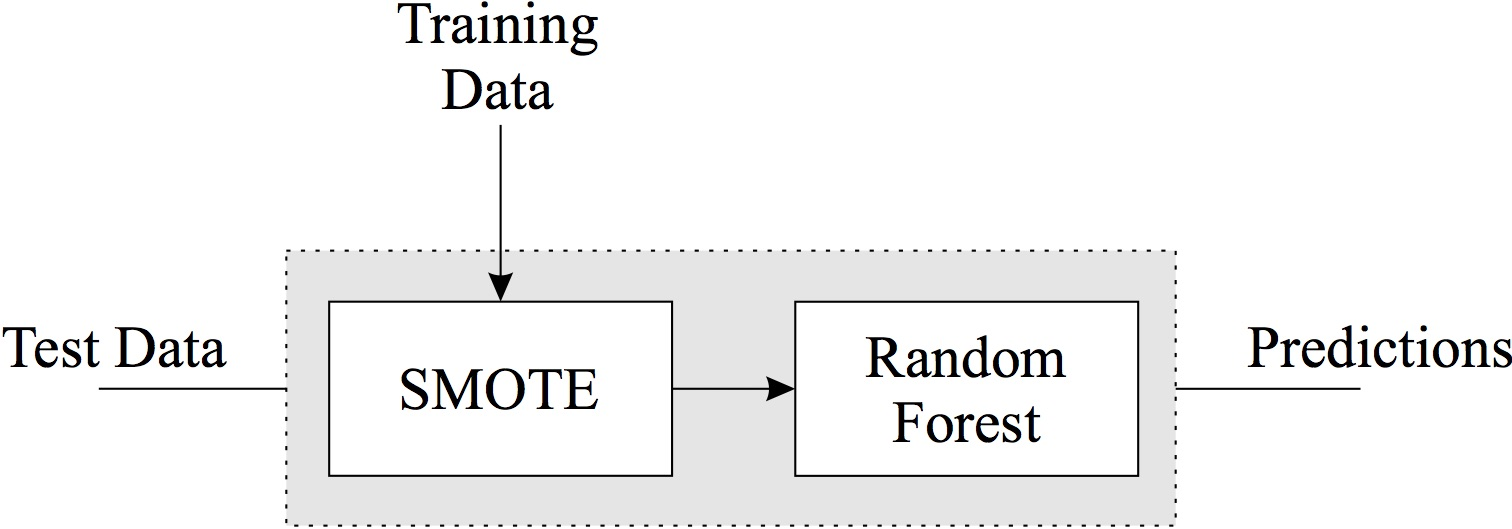
\includegraphics[width=\linewidth]{./_figs/Oracle}}\\
  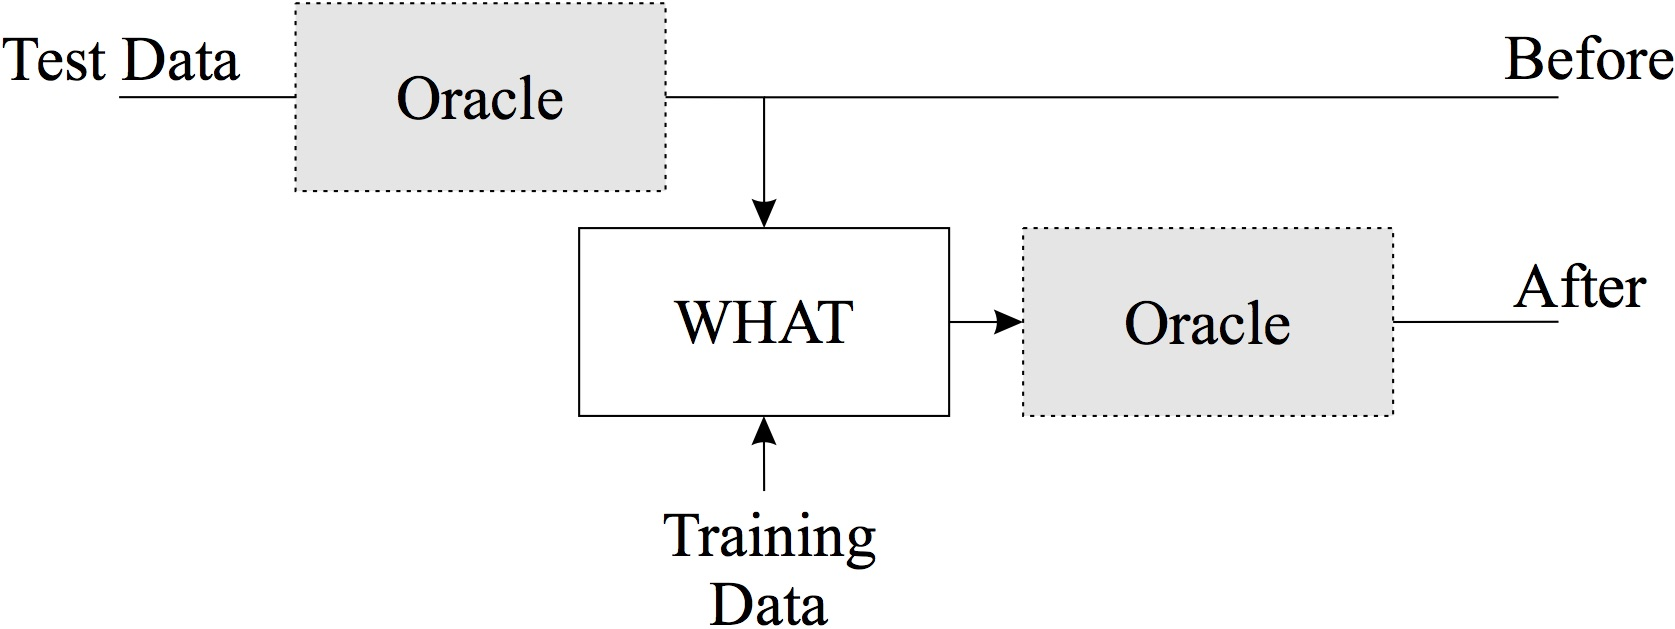
\includegraphics[width=\linewidth]{./_figs/WHAT}
  \caption{The Planning scheme}
  \label{fig:what}
\end{figure}

%involves two key components. Firstly, there is the oracle (Random Forest with SMOTE) which is used to make predictions. Then we have the 
\subsection{Data sets}
The data was obtained from the PROMISE repository. For the defect data we investigated 32 releases from 11 open source Java projects defined by the metrics highlighted in Fig.~\ref{fig:ck}: \kw{Apache Ant} (1.5 -- 1.7), \kw{Apache Camel} (1.2 -- 1.6), \kw{Apache Ivy} (1.1 -- 2.0), \kw{JEdit} (4.1 -- 4.3), \kw{Apache Log4j} (1.0 -- 1.2), \kw{Apache Lucene} (2.0 -- 2.2), \kw{PBeans} (1.0 and 2.0), \kw{Apache POI} (2.0 -- 3.0), \kw{Apache Synapse} (1.0 -- 1.2), \kw{Apache Velocity} (1.4 -- 1.6), and \kw{Apache Xalan-Java} (2.5 -- 2.7). Given the empirical nature of the data, it is important to design an experiment such that the planning phase uses only the \kw{past} data to learn trends which can then be applied to the \kw{future} data. Thus for our experiment we use data sets that have at least two consecutive releases. 
\begin{itemize}
\item To generate recommendations for a release $i$, the planner uses releases releases $(i-1)$ and $(i-2)$.
\item The predictor also uses releases $(i-1)$ and $(i-2)$. However, we use SMOTE with re-sampling in order to handle the class imbalance in the data and to prevent the predictor from using the same training data as the planner.
\end{itemize}


In order to answer {\bfseries RQ4}, we have used the performance prediction data set was obtained from the PROMISE repository~\cite{}. The data set contains six examples of real world configurable systems: \kw{Apache}, \kw{LLVM}, \kw{x264}, \kw{Berkeley DB (written in C and Java}, and \kw{SQLite}. The systems have different characteristics, different implementation languages, and different configuration mechanisms. The data set is a collection of all possible configurations (with SQLITE being a exception with only 4653 configurations). 

\subsection{The Rig}

The experimental rig is shown in Figure \ref{fig:rig}. It uses an \textit{oracle} to determine wether a certain test case is defective or not. If the oracle suggests that an instance is defective, then we use WHAT to apply the recommendations to that test instance. The oracle is used to check if the recommendation helped subdue the defect.

\subsection{Performance Assessment}

In order to assess the performance of the planner for the defect data set, we use the Cliffs Delta score to measure the probability that the number of bugs in test data before applying the planner is larger than after doing so. In other words, we use the delta score to measure the ability of the planner to effective reduce the number of defects. Given the untreated test instance labeled \textit{Before} of length \textit{M} and the treated instances labeled \textit{After}, the delta score is obtained as follows:
\begin{equation}
\delta = \frac{\#(Before>After) - \#(Before<After)}{M^2}
\end{equation}

In the context of our application, the $\delta$ attains a value of 1 if the number of defects after applying the treatments has reduced to zero, and 0 if there is no change.

For the performance prediction data set on the other hand, Cliff's delta measure is not directly applicable. We therefore assess the performance by measuring the gain, given by $\frac{Before}{After}$. The gain takes a value larger than 1 if the run times have been reduced, a value of 1 if there is no change, and a value less than 1 if run times have increased after applying the recommended changes. 

In addition to the above, we rank the different variants of the planning scheme to identify the best approach. We make use of the Scott-Knott procedure, recommended by Mittas \& Angelis in their 2013 IEEE TSE paper~\cite{sk}, to compute the ranks. It works as follows: A list of treatments \textit{l} is sorted by the Medianian score. The list \textit{l} is then split into sub-lists m, n in order to maximize the expected value of the differences in the observed performance before and after division. A statistical hypothesis test \textit{H} is applied on the splits \textit{m, n} to check if they are statistically different. If so, Skott-Knott then recurses on each division. 

The research conducted by Shepperd and MacDonell~\cite{shepperd12a}, Kampenes~\cite{kampenes07} and Kocaguenli et al.~\cite{}, highlighted that an ``effect size'' in lieu of a mere hypothesis test is required in order to verfiy if two populations are ``significantly'' different. An ICSE'11 paper by Arcuri~\cite{} endorsed the use of Vargha and Delaney's A12 effect size for reporting results in software engineering. Thus, for hypothesis testing H in Skott-Knott, we use the A12 test and a non-parametric bootstrap sampling~\cite{}.

\section{Experimental Results}
\begin{figure}[!t]
\centering
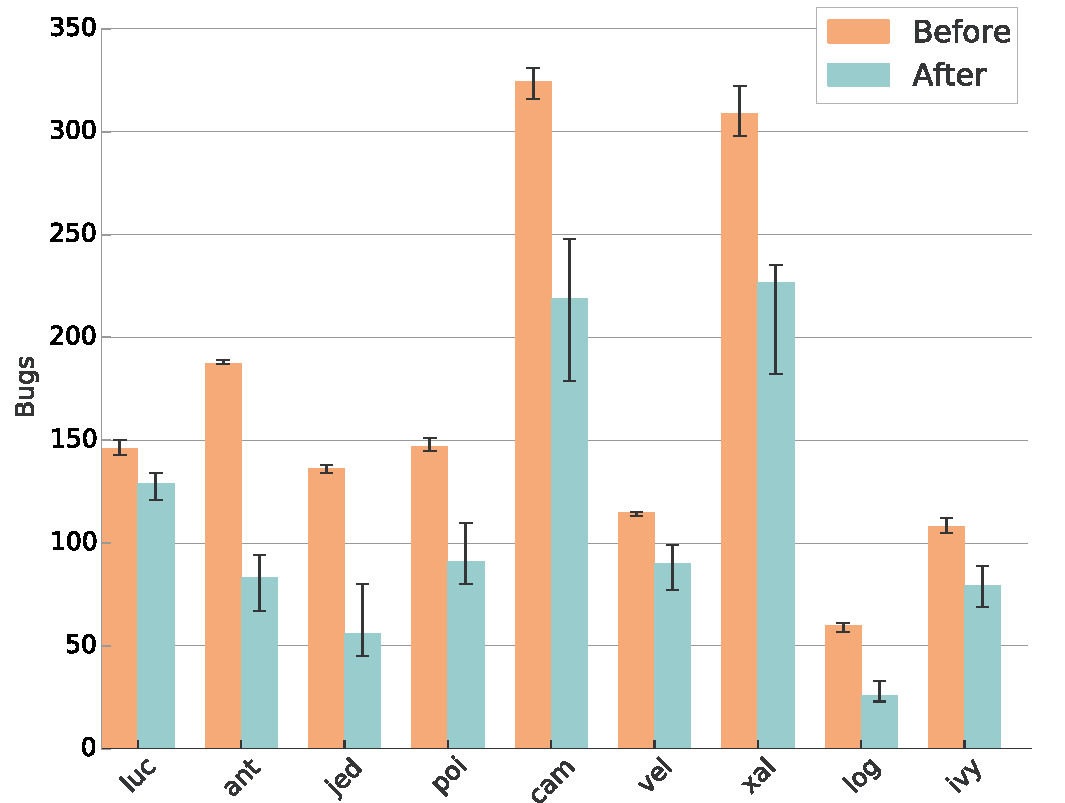
\includegraphics[width=\linewidth]{_figs/histograms.pdf}
\caption{Caption}
\label{fig:bugs}
\end{figure}

\begin{figure*}[htbp!]

\noindent\begin{minipage}{0.5\textwidth}
  {\scriptsize \textbf{Ant}\\}
  {\scriptsize  \begin{tabular}{{l@{~~~~}l@{~~~~}r@{~~~~}r@{~~~~}c}}
      \arrayrulecolor{darkgray}
      \rowcolor[gray]{.9} \textbf{Rank} & \textbf{Treatment} & \textbf{Median} & \textbf{IQR} & \\\hline
      1 &     Base &    0.13  &  0.03 & \quart{0}{1}{1}{48}\\
      \hline  2 & 0.25, weighting,  iP=50\% &    0.2  &  0.05 & \quart{3}{3}{4}{48}\\
      \hline  3 & 0.5, weighting,  iP=50\% &    0.26  &  0.06 & \quart{6}{3}{8}{48}\\
      \hline  4 &     0.25 &    0.3  &  0.1 & \quart{7}{6}{10}{48}\\
      4 &   0.25, weighting&    0.3  &  0.08 & \quart{8}{4}{10}{48}\\
      \hline  5 & 0.75, weighting,  iP=50\% &    0.42  &  0.13 & \quart{13}{7}{17}{48}\\
      5 &      0.5 &    0.43  &  0.1 & \quart{14}{6}{17}{48}\\
      5 &    0.5, weighting&    0.43  &  0.1 & \quart{15}{5}{17}{48}\\
      \hline  6 &   0.75, weighting&    0.64  &  0.19 & \quart{22}{10}{29}{48}\\
      6 &     0.75 &    0.63  &  0.08 & \quart{26}{4}{28}{48}\\
      \hline \end{tabular}}
\end{minipage}
\noindent\begin{minipage}{0.5\textwidth}
  \flushleft
  {\scriptsize \textbf{Camel}\\}
{\scriptsize  \begin{tabular}{{l@{~~~~}l@{~~~~}r@{~~~~}r@{~~~~}c}}
\arrayrulecolor{darkgray}
\rowcolor[gray]{.9} \textbf{Rank} & \textbf{Treatment} & \textbf{Median} & \textbf{IQR} & \\\hline
  1 &   Base &    0.15  &  0.05 & \quart{0}{4}{1}{75}\\
\hline  2 &   0.25 &    0.18  &  0.06 & \quart{1}{5}{4}{75}\\
  2 & 0.25, weighting&    0.2  &  0.06 & \quart{2}{5}{6}{75}\\
  2 & 0.25, weighting,  iP=50\% &    0.2  &  0.04 & \quart{4}{3}{6}{75}\\
\hline  3 &  0.5, weighting&    0.25  &  0.1 & \quart{6}{9}{10}{75}\\
  3 &    0.5 &    0.26  &  0.12 & \quart{6}{11}{11}{75}\\
  3 & 0.5, weighting,  iP=50\% &    0.28  &  0.11 & \quart{10}{9}{13}{75}\\
\hline  4 & 0.75, weighting&    0.39  &  0.16 & \quart{19}{13}{22}{75}\\
  4 &   0.75 &    0.42  &  0.17 & \quart{15}{15}{25}{75}\\
  4 & 0.75, weighting,  iP=50\% &    0.42  &  0.1 & \quart{20}{9}{25}{75}\\
\hline \end{tabular}}
\end{minipage}

\noindent\begin{minipage}{0.5\textwidth}
  \flushleft
  {\scriptsize \textbf{Ivy}\\[-0.05cm]}
{\scriptsize  \begin{tabular}{{l@{~~~~}l@{~~~~}r@{~~~~}r@{~~~~}c}}
\arrayrulecolor{darkgray}
\rowcolor[gray]{.9} \textbf{Rank} & \textbf{Treatment} & \textbf{Median} & \textbf{IQR} & \\\hline
  1 & 0.25, weighting,  iP=50\% &    0.15  &  0.04 & \quart{0}{2}{0}{55}\\
\hline  2 &     Base &    0.16  &  0.0 & \quart{1}{0}{1}{55}\\
  2 &     0.25 &    0.18  &  0.06 & \quart{1}{4}{2}{55}\\
  2 &   0.25, weighting&    0.2  &  0.06 & \quart{1}{4}{3}{55}\\
\hline  3 & 0.5, weighting,  iP=50\% &    0.28  &  0.08 & \quart{7}{5}{9}{55}\\
\hline  4 &      0.5 &    0.33  &  0.11 & \quart{8}{7}{12}{55}\\
  4 &    0.5, weighting&    0.37  &  0.09 & \quart{10}{6}{14}{55}\\
\hline  5 & 0.75, weighting,  iP=50\% &    0.38  &  0.16 & \quart{12}{10}{15}{55}\\
\hline  6 &   0.75, weighting&    0.56  &  0.08 & \quart{25}{5}{27}{55}\\
  6 &     0.75 &    0.57  &  0.12 & \quart{25}{7}{27}{55}\\[-0.01cm]
\hline \end{tabular}}
\end{minipage}
\noindent\begin{minipage}{0.5\textwidth}
  \flushleft
  {\scriptsize \textbf{Jedit}\\}
  {\scriptsize  \begin{tabular}{{l@{~~~~}l@{~~~~}r@{~~~~}r@{~~~~}c}}
\arrayrulecolor{darkgray}
\rowcolor[gray]{.9} \textbf{Rank} & \textbf{Treatment} & \textbf{Median} & \textbf{IQR} & \\\hline
  1 &   Base &    0.06  &  0.01 & \quart{0}{0}{0}{64}\\
\hline  2 & 0.25, weighting&    0.08  &  0.06 & \quart{0}{4}{1}{64}\\
  2 &   0.25 &    0.09  &  0.05 & \quart{0}{3}{2}{64}\\
\hline  3 & 0.25, weighting,  iP=50\% &    0.12  &  0.08 & \quart{1}{5}{4}{64}\\
\hline  4 &  0.5, weighting&    0.16  &  0.09 & \quart{4}{6}{6}{64}\\
  4 &    0.5 &    0.17  &  0.09 & \quart{4}{6}{7}{64}\\
\hline  5 & 0.5, weighting,  iP=50\% &    0.22  &  0.11 & \quart{8}{8}{10}{64}\\
  5 & 0.75, weighting&    0.26  &  0.18 & \quart{9}{12}{13}{64}\\
\hline  6 &   0.75 &    0.38  &  0.31 & \quart{11}{21}{21}{64}\\
  6 & 0.75, weighting,  iP=50\% &    0.41  &  0.17 & \quart{17}{12}{24}{64}\\
\hline \end{tabular}}
\end{minipage}


\noindent\begin{minipage}{0.5\textwidth}
  \flushleft
  {\scriptsize \textbf{Log4j}\\}
  {\scriptsize  \begin{tabular}{{l@{~~~~}l@{~~~~}r@{~~~~}r@{~~~~}c}}
\arrayrulecolor{darkgray}
\rowcolor[gray]{.9} \textbf{Rank} & \textbf{Treatment} & \textbf{Median} & \textbf{IQR} & \\\hline
  1 &   Base &    0.06  &  0.03 & \quart{0}{4}{4}{139}\\
\hline  2 & 0.25, weighting&    0.09  &  0.04 & \quart{4}{6}{8}{139}\\
  2 &   0.25 &    0.09  &  0.06 & \quart{4}{8}{8}{139}\\
  2 & 0.25, weighting,  iP=50\% &    0.09  &  0.04 & \quart{4}{6}{8}{139}\\
  2 &    0.5 &    0.1  &  0.07 & \quart{4}{10}{10}{139}\\
\hline  3 &  0.5, weighting&    0.12  &  0.03 & \quart{10}{4}{12}{139}\\
\hline  4 & 0.75, weighting&    0.13  &  0.11 & \quart{10}{15}{14}{139}\\
  4 &   0.75 &    0.13  &  0.06 & \quart{12}{9}{14}{139}\\
  4 & 0.5, weighting,  iP=50\% &    0.13  &  0.06 & \quart{10}{8}{14}{139}\\
\hline  5 & 0.75, weighting,  iP=50\% &    0.19  &  0.11 & \quart{17}{15}{22}{139}\\
\hline \end{tabular}}
\end{minipage}
\noindent\begin{minipage}{0.5\textwidth}
  \flushleft
  {\scriptsize \textbf{Lucene}\\}
  {\scriptsize  \begin{tabular}{{l@{~~~~}l@{~~~~}r@{~~~~}r@{~~~~}c}}
\arrayrulecolor{darkgray}
\rowcolor[gray]{.9} \textbf{Rank} & \textbf{Treatment} & \textbf{Median} & \textbf{IQR} & \\\hline
  1 &  0.25 &    0.05  &  0.02 & \quart{1}{4}{3}{188}\\
  1 & 0.25, weighting&    0.05  &  0.04 & \quart{0}{7}{3}{188}\\
\hline  2 &   0.5 &    0.07  &  0.04 & \quart{3}{8}{7}{188}\\
  2 & 0.25, weighting,  iP=50\% &    0.07  &  0.04 & \quart{3}{8}{7}{188}\\
  2 & 0.5, weighting&    0.08  &  0.05 & \quart{5}{10}{9}{188}\\
\hline  3 & 0.5, weighting,  iP=50\% &    0.1  &  0.03 & \quart{9}{6}{13}{188}\\
  3 &  Base &    0.1  &  0.03 & \quart{7}{6}{13}{188}\\
\hline  4 & 0.75, weighting,  iP=50\% &    0.13  &  0.09 & \quart{9}{18}{19}{188}\\
  4 &  0.75 &    0.15  &  0.08 & \quart{13}{16}{23}{188}\\
  4 & 0.75, weighting&    0.15  &  0.11 & \quart{11}{21}{23}{188}\\
\hline \end{tabular}}
\end{minipage}

\noindent\begin{minipage}{0.5\textwidth}
  \flushleft
  {\scriptsize \textbf{Poi}\\}
  {\scriptsize  \begin{tabular}{{l@{~~~~}l@{~~~~}r@{~~~~}r@{~~~~}c}}
      \arrayrulecolor{darkgray}
\rowcolor[gray]{.9} \textbf{Rank} & \textbf{Treatment} & \textbf{Median} & \textbf{IQR} & \\\hline
  1 &     Base &    0.1  &  0.03 & \quart{0}{2}{1}{61}\\
\hline  2 & 0.25, weighting,  iP=50\% &    0.14  &  0.1 & \quart{0}{6}{4}{61}\\
\hline  3 &   0.25, weighting&    0.18  &  0.14 & \quart{4}{9}{6}{61}\\
  3 &     0.25 &    0.19  &  0.11 & \quart{4}{7}{7}{61}\\
  3 & 0.5, weighting,  iP=50\% &    0.2  &  0.19 & \quart{4}{13}{8}{61}\\
\hline  4 & 0.75, weighting,  iP=50\% &    0.26  &  0.2 & \quart{8}{13}{12}{61}\\
  4 &      0.5 &    0.28  &  0.2 & \quart{6}{14}{13}{61}\\
  4 &    0.5, weighting&    0.33  &  0.22 & \quart{10}{14}{16}{61}\\
\hline  5 &     0.75 &    0.47  &  0.22 & \quart{18}{14}{26}{61}\\
  5 &   0.75, weighting&    0.46  &  0.11 & \quart{22}{7}{25}{61}\\
\hline \end{tabular}}
\end{minipage}
\noindent\begin{minipage}{0.5\textwidth}
  \flushleft
  {\scriptsize \textbf{Synapse}\\}
  {\scriptsize  \begin{tabular}{{l@{~~~~}l@{~~~~}r@{~~~~}r@{~~~~}c}}
\arrayrulecolor{darkgray}
\rowcolor[gray]{.9} \textbf{Rank} & \textbf{Treatment} & \textbf{Median} & \textbf{IQR} & \\\hline
  1 & Base &    0.15  &  0.0 & \quart{1}{0}{1}{44}\\
  1 & 0.5, weighting,  iP=50\% &    0.15  &  0.08 & \quart{1}{4}{1}{44}\\
  1 & 0.25, weighting,  iP=50\% &    0.17  &  0.08 & \quart{0}{4}{2}{44}\\
\hline  2 & 0.75, weighting,  iP=50\% &    0.21  &  0.08 & \quart{1}{4}{4}{44}\\
  2 & 0.25 &    0.23  &  0.18 & \quart{2}{9}{5}{44}\\
  2 & 0.25, weighting&    0.23  &  0.11 & \quart{2}{5}{5}{44}\\
\hline  3 & 0.5, weighting&    0.38  &  0.19 & \quart{7}{10}{12}{44}\\
  3 &  0.5 &    0.42  &  0.27 & \quart{6}{14}{14}{44}\\
\hline  4 & 0.75 &    0.5  &  0.39 & \quart{12}{20}{19}{44}\\
  4 & 0.75, weighting&    0.56  &  0.25 & \quart{17}{12}{22}{44}\\
\hline \end{tabular}}
\end{minipage}

\noindent\begin{minipage}{0.50\textwidth}
  \flushleft
  {\scriptsize \textbf{Velocity}\\}
  {\scriptsize  \begin{tabular}{{l@{~~~~}l@{~~~~}r@{~~~~}r@{~~~~}c}}
\arrayrulecolor{darkgray}
\rowcolor[gray]{.9} \textbf{Rank} & \textbf{Treatment} & \textbf{Median} & \textbf{IQR} & \\\hline
  1 & 0.25, weighting,  iP=50\% &    0.03  &  0.06 & \quart{0}{5}{1}{98}\\
  1 & 0.25 &    0.04  &  0.02 & \quart{1}{2}{2}{98}\\
  1 & 0.25, weighting&    0.05  &  0.03 & \quart{2}{3}{3}{98}\\
  1 & Base &    0.05  &  0.06 & \quart{0}{5}{3}{98}\\
\hline  2 & 0.5, weighting,  iP=50\% &    0.07  &  0.11 & \quart{3}{11}{5}{98}\\
  2 & 0.5, weighting&    0.1  &  0.08 & \quart{5}{8}{8}{98}\\
\hline  3 & 0.5 &    0.13  &  0.12 & \quart{5}{12}{11}{98}\\
\hline  4 & 0.75 &    0.16  &  0.24 & \quart{8}{24}{14}{98}\\
  4 & 0.75, weighting,  iP=50\% &    0.17  &  0.15 & \quart{9}{15}{15}{98}\\
  4 & 0.75, weighting&    0.22  &  0.22 & \quart{9}{22}{20}{98}\\
\hline \end{tabular}}
\end{minipage}
\noindent\begin{minipage}{0.50\textwidth}
  \flushleft
  {\scriptsize \textbf{Xalan}\\}
  {\scriptsize  \begin{tabular}{{l@{~~~~}l@{~~~~}r@{~~~~}r@{~~~~}c}}
\arrayrulecolor{darkgray}
\rowcolor[gray]{.9} \textbf{Rank} & \textbf{Treatment} & \textbf{Median} & \textbf{IQR} & \\\hline
  1 &   Base &    0.08  &  0.02 & \quart{0}{1}{0}{80}\\
\hline  2 & 0.5, weighting,  iP=50\% &    0.14  &  0.05 & \quart{3}{4}{6}{80}\\
  2 & 0.75, weighting,  iP=50\% &    0.15  &  0.06 & \quart{5}{5}{6}{80}\\
  2 & 0.25, weighting,  iP=50\% &    0.15  &  0.06 & \quart{3}{5}{6}{80}\\
\hline  3 &   0.25 &    0.23  &  0.11 & \quart{8}{10}{13}{80}\\
  3 & 0.25, weighting&    0.23  &  0.09 & \quart{10}{8}{13}{80}\\
\hline  4 &  0.5, weighting&    0.28  &  0.06 & \quart{16}{5}{18}{80}\\
\hline  5 &    0.5 &    0.3  &  0.13 & \quart{15}{11}{19}{80}\\
  5 & 0.75, weighting&    0.34  &  0.19 & \quart{16}{16}{23}{80}\\
  5 &   0.75 &    0.38  &  0.11 & \quart{21}{10}{26}{80}\\
\hline \end{tabular}}
\end{minipage}
   \end{figure*}


% \section{Discussion}
% \section{Threats to validity}
% \section{Conclusion}
% \section*{Acknowledgements}
\newpage
\bibliography{References}{}
\bibliographystyle{IEEEtran}
\end{document}
